% Master LaTex file for gyarb

% Shortcuts
% C-c C-c compile
% Compile
% 1: pdflatex garb_bokma.tex, 2:makeglossaries garb_bokma, 3: biber garb_bokma, 4: pdflatex garb_bokma.tex


\documentclass[11pt]{article}

% packages
\usepackage[margin=1in]{geometry}
\usepackage[backend=biber]{biblatex}
\usepackage{graphicx}
\usepackage{wrapfig}
\usepackage{csvsimple}
\usepackage[toc, acronym]{glossaries}
\usepackage{comment}
\usepackage{hyperref}

% settings
\addbibresource{garb_bibl.bib}
\hypersetup{
    colorlinks=true,
    linkcolor=black,
    filecolor=black,
    urlcolor=blue,
    citecolor=black
  }

% title
\title{Predicting long term effects if TBI using machine learning}
\author{Author: Otte Bokma\\
Supervisor: Lars Burström}

% glossary
\makeglossaries
\newglossaryentry{drd2}
{
  name = Gene dopamine receptor D2,
  description = {DRD2 is a gene thet codes the dopamine receptor D2 that is the target for a variety of psychotrpic agents\cite{DRD2SNPedia}}
}
\newglossaryentry{ankk1}
{
  name = Gene ankyrin repeat and kinase domain containing 1,
  description = {ANKK1 is a gene that codes for the ANKK1 enzyme \cite{ANKK12020}}
}
\newglossaryentry{COMT}
{
  name = Gene catechol-O-methyltransferase gene,
  description = {The COMT gene is a gene in which variations affect dopamine levels in the prefrontal cortex\cite{comtsnpedia}. The gene codes for catechol-O-Methyltransferase, an enzyme that breaks down dopamine in the prefrontal cortex\cite{Rs4680snpedia}.}
}
\newglossaryentry{TBI}
{
  name = Traumatic Brain Injury,
  description = {Brain injury cause by trauma to the head},
  plural= traumatic brain injuries
}
\newglossaryentry{GOSE}
{
  name = Extended Glasgow Outcome Scale,
  description = {Method for classifying outcome of traumatic brain injury}
}
\newglossaryentry{bc}
{
  name = basal/cerebral/subarachnoid cistern,
  description = {Space formed by openings between the \gls{pm} and \gls{am} that are filled with \gls{csf}\cite{SubarachnoidCisterns2020}\cite{CerebralCisternsWRadiology2020}}
}
\newglossaryentry{csf}
{
  name = cerebrospinal fluid,
  description = {Clear, colorless fluid surrounding the brain and spinal chord acting as a cushing and buffer for both mechanical and immunological protection of the brain and spine\cite{CerebrospinalFluid2021}}
}
\newglossaryentry{men}
{
  name = meninx,
  description = {the meninges are three membranes enveloping the brain ans spinal chord. In mammals consisting of the \gls{dm}, \gls{am} and \gls{pm}\cite{Meninges2021}}
  plural = meninges
}
\newglossaryentry{am}
{
  name = arachnoid mater,
  description = {A membrane which along with the \gls{dm} and pia mater cover and protect the brain and spinal chord\cite{ArachnoidMater2021}}
}
\newglossaryentry{dm}
{
  name = dura mater,
  description = {A thick membrane of dense irregular connective tissue surrounding the brain and spinal chord\cite{DuraMater2021}}
}
\newglossaryentry{pm}
{
  name = pia mater,
  description = {The innermost layer of the \glspl{men}\cite{PiaMater2021}}
}
\newglossaryentry{bv}
{
  name = bridging vein,
  description = {Veins in the meninges that go through the \gls{dm} and empty into the \glspl{dvs}\cite{BridgingVein2020}}
}
\newglossaryentry{dvs}
{
  name = dural venous sinus,
  description = {venous channels between the meninges and endosteum\cite{DuralVenousSinuses2020}},
  plural = dural venous sinuses
}
\newglossaryentry{mma}
{
  name = middle meningeal artery,
  description = {The largest of three (paired) arteries that supply the \gls{men} with blood\cite{MiddleMeningealArtery2021}},
}
\newglossaryentry{susp}
{
  name = subarachnoid space,
  description = {Area between the \gls{am} and the \gls{pm} surrounding the brain\cite{jonesSubarachnoidSpaceRadiology}}
}
\newglossaryentry{ca}
{
  name = cerebral aneurysm,
  description = {Weakness in the wall of a cerebral artery or vein causing dilation of the blood vessels\cite{IntracranialAneurysm2021}}
}
\newglossaryentry{bh}
{
  name = brain herniation,
  description = {An effect of high pressure within the skull that puts high pressure on parts of the brain which leads to insufficient blood supply to parts of the brain as blood vessels are constricted. The cause is that a part of the brain is pushed across structures in the skull. Brain herniation is often fatal. \cite{BrainHerniation2020}}
}
\newglossaryentry{icp}
{
  name = intracranial pressure,
  description = {Pressure inside the skull exerted by fluids\cite{IntracranialPressure2021}}
}
\newglossaryentry{hc}
{
  name = hydrocephalus,
  description = {A contidion that causes accumulation of \gls{csf} in the brain that often causes increased \gls{icp}\cite{Hydrocephalus2021}}
}
\newacronym{ptsd}{PTSD}{post traumatic stress disorder}
\newacronym{tsah}{tSAH}{traumatic subarachnoid hemorrhage}
\newacronym{snp}{SNP}{single nucleotide polymorphism}
\newacronym{comt}{COMT}{catechol-O-methyltransferase}
\newacronym{sah}{SAH}{subarachnoid hemorrhage}
\newacronym{sh}{SH}{subdural hematoma}
\newacronym{mmc}{MMC}{maximal margin classifier}
\newacronym{svc}{SVC}{support vector classifier}
\newacronym{svm}{SVM}{support vector machine}
\newacronym{rbf}{RBF}{radial basis function kernel}
\newacronym{tbi}{TBI}{traumatic brain injury}
\newacronym{gose}{GOSE}{extended Glasgow outcome scale}
\newacronym{ct}{CT}{computed tomography}
\newacronym{cns}{CNS}{central nervous system}
% document
\begin{document}

\begin{titlepage}
\maketitle
\end{titlepage}

\begin{comment}
\section*{Sammanfattning}

Hjärnskakningar är relativt vanliga skador och framkommer framför allt bland idrottare inom vissa sporter, exempelvis ishockey\cite{TraumaticBrainInjury}. Det finns olika former av hjänskakningar och symptomen varierar på både lång och kort sikt mellan fallen. En del personer påverkas nästan inte medan andra kan få problem som varar i många år. Att förutsäga de långvariga symptomen kan därför vara svårt.\cite{TraumaticBrainInjury2021}\\
\\
Maskininlärning kan användas för att identifiera eller förutsäga något utifrån olika variabler\cite{MachineLearning2021}. Det skulle vara tänkbart att artificiell intelligens skulle kunna förutsäga möjliga långvariga symptom av en hjärnskaknings skador en person fått utifrån olika variabler.\\
\\
Maskininlärningsmetoden som användes var en så kallad \gls{svm}. Den kördes med olika kernel funktioner vilka ändrar hur algoritmed delar in datan i klasser\cite{KernelMethod2021}.\cite{jamesSupportVectorMachines}\\
\\
Rotterdam och Marshall CT score kunde förutsägas någorlunda tillförlitligt med en \gls{svm} och patienters skador som faktorer. 6 månaders \gls{ptsd} och \gls{gose} poäng för patientens resultat kunde inte förutsägas tillförlitligt. Varken med Marshall och Rotterdam CT score som faktorer eller tillsammans med genetiska faktorer.
\end{comment}

\section*{Abstract}

\Gls{tbi} is a relatively common condition, especially among athletes of some sports, such as ice-hockey\cite{TraumaticBrainInjury}. There are different types of \gls{tbi} and the symptoms can vary in both long term and short term. To predict the long term effects of \gls{tbi} can therefore be hard. Some people have almost no long term symptoms whilst others may have symptoms years after the accident occurred.\cite{TraumaticBrainInjury2021}\\
\\
Machine learning has been shown to be suitable for this type of application, to identify or pedict possible outcomes based on a set of variables\cite{MachineLearning2021}. The variables in this case being the injuries that patients have received. It could thus be conceivable that possible long term effects caused by \gls{tbi} could be predicted.\\
\\
Machine learning is a very broad term meaning any algorithm that makes a model based on sample data which it then uses to make predictions about other data. In this case the type of machine learning algorithm used is a \gls{svm}, as it performs well for many types of settings without needing a lot of optimization for a specific use-case. The classifier was run on several different kernel functions which change how the algorithm divides data into classes\cite{KernelMethod2021}.\cite{jamesSupportVectorMachines}\\
\\
The algorithm was run to predict two patient outcome predictors (Rotterdam and Marshall \gls{ct} scores) based on the injuries a patient had received, and two patient outcome scores (6 month \gls{gose} and \gls{ptsd}) based on the patients outcome predictors and on some genetic factors that have a possile link to the outcome in cases of \gls{tbi}.\\
\\
The Rotterdam and Marshall \gls{ct} scores could be somewhat reliably predicted. The 6 month \gls{gose} and \gls{ptsd} scores for patient outcome could not be reliably predicted. Neither using the Marshall and Rotterdam CT scores on their own or along with genetic factors.



\section*{Restrictions}
The focus of the study lies in trying to use a support vector machine to predict the long term effects of traumatic brain injury. Therefore some restrictions have to be made regarding the math and algorithms behind the support vector machine as explaining it lies beyond the scope of this study.

\section*{Keywords}
Support Vector Machine, Brain Injury, Machine Learning

\newpage
\tableofcontents
\newpage
\section{Introduction}
Traumatic brain injury (\gls{tbi}) is a condition that can be quite hard to diagnose and even if diagnosed the long term effects and symptoms can be hard to identify. This is because there are different types of \gls{tbi} and the symptoms can vary both short term and long term. To predict the effects of \gls{tbi} can therefore be hard. Some people have almost no symptoms while others may have symptoms years after the accident occurred.\cite{TraumaticBrainInjury2021}\cite{TraumaticBrainInjury}\\
\\
\gls{tbi} is frequently caused by and a relatively common injury in traffic accidents, physical violence and falls and has a varying presence depending on a persons daily activities. In more than others \gls{tbi} shows among athletes of some sports, such as boxing, American football and ice-hockey\cite{TraumaticBrainInjury}.\cite{TraumaticBrainInjury2021}\\
\\
Machine learning has in recent times gained popularity as it gives a way of identifying and predicting things humans cannot always do, and as such it is used widely for varying kinds of applications. It has been shown to be suitable for applications, such as this, where something is identified or predicted based on a set of variables. In this case the variables being the injuries that patients have received and other data possibly linked with \gls{tbi} outcome, which are then used to predict the long term effects caused by their injuries. It could thus be conceived that long term effects caused by \gls{tbi} could be predicted.\cite{ArtificialIntelligence2021a}\cite{MachineLearning2021}\\
\\
As for \gls{TBI} there is a lot of data to be collected about a patients health status at the time of being examined. This data is quite hard for humans to interpret. Using machine learning to interpret this data has the potential to use its capabilities of data classification.\cite{TraumaticBrainInjury2021}\cite{nielsonUncoveringPrecisionPhenotypebiomarker2017}

\subsection*{Purpose}
The purpose of the study is to try to answer the following questions:

\begin{enumerate}
  \item{How accurately can the Marshall and Rotterdam classifications be predicted with data of the injuries a patient has suffered.}
  \item{How well do the Marshall and Rotterdam classifications predict \gls{ptsd} and the score of the Extended Glasgow Outcome Scale}
  \item{Can a correlation between genetic factors and patient outcome (\gls{gose} and \gls{ptsd}) be found using machine learning}
\end{enumerate}

\section{Background}
The type of machine learning algorithm used is a \gls{svm}, which have been shown to perform well in many different settings and are considered to be one of the best classifiers to use without considerable optimization for a specific classification problem. The exact algorithm used was the support vector machine from scikit-learn\cite{SklearnSvmSVC}\cite{pedregosaScikitlearnMachineLearning2011}.\\
\\
The classification was conducted by separating data values into features (used for predicting the label) and labels (predicted using features). The features and labels are then divided into training data and test data. In this case the training data consists of 80\% of all data and the test data consists of 20\%. The training data is what the algorithm uses to make a model of a function by which is considers the data to be separable, then this model is tested on the test data and scored by the percentile of correct  classifications.\\
\\
The separation of data into training and test data is done for each iteration of running the algorithm and each time the datapoints are separated the datapoints are used for each group are randomize. Thus the data used for training and prediction is not the same every time which means that also the results vary for each iteration of running the algorithm. To make the results more reliable the program runs 3000 iterations for the division of the data, and the algorithm. The score for each iteration is calculated and added to a variable, after which the total sum is divided by the number of iterations to get the average score.\\
\\
Results from a few of the iterations are also analyzed manually to see what kind of predictions the algorithm makes. A great part of the label classes are concentrated to just one or two of the classes, meaning that the algorithm can get a score that is quite high by just classifying all labels into one or two classes.

\subsection{Support Vector Machines}
The support vector machine, or SVM, is a generalization of a classifier called the \textit{maximal margin classifier}. This classifier however, can not be applied to most datasets as it requires classes to be separable by a linear boundary. With the use of the \textit{support vector classifier}, which is an extension of the of the maximal margin classifier, SVMs become applicable to more datasets. The \textit{support vector machine} is a further extension of the \textit{support vector classifier} that accommodates for class boundaries that are non-linear. Even further extensions can be made to the \textit{support vector machine} to make it applicable to more than two classes.\cite{jamesSupportVectorMachines}\\
\\
It is important to distinguish between the \textit{maximal margin classifier}, \textit{support vector classifier} and \textit{support vector machine}, as not to confuse them with each other.\cite{jamesSupportVectorMachines}

\subsubsection{Kernels}
Kernels are similarity functions. A similarity functions objective is to calculate the similarity between objects. Using a kernel means that we can add dimensions so that the data gets separable into classes. The use of a kernel implies the use of a kernel function, that enables the use of high-dimensional space without needing to compute the coordinates of the data in that space. Instead it calculates the inner (dot) product for all pairs of images of data.\cite{KernelMethod2021}\\
\\
The type of kernel used defines what kind of function is used to make the model for separating the data into different classes.\cite{SVMKernelsScikitlearn24}\\
\\
Figures 1, 2, and 3 illustrate the use of a linear, radial basis function, and polynomial kernel respectively.

\begin{figure}[ht]
  \centering
  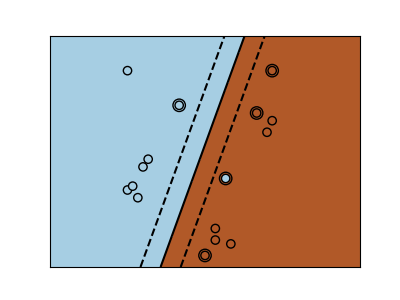
\includegraphics[width=12cm]{graphics/kernel_linear.png}
  \caption{Figure showing a linear kernel\cite{SVMKernelsScikitlearn24}}
\end{figure}

\begin{figure}[ht]
  \centering
  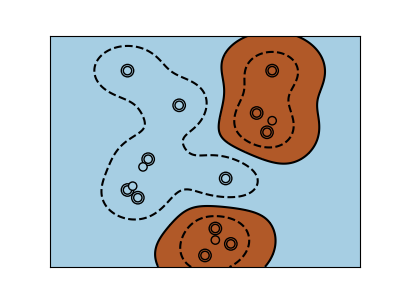
\includegraphics[width=12cm]{graphics/kernel_rbf.png}
  \caption{Figure showing a radial basis function kernel\cite{SVMKernelsScikitlearn24}}
\end{figure}

\begin{figure}[ht]
  \centering
  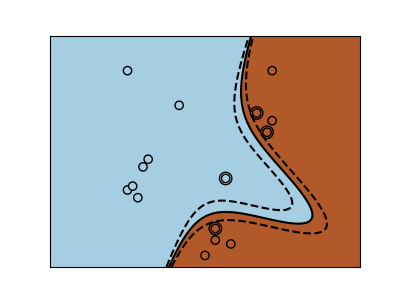
\includegraphics[width=12cm]{graphics/kernel_poly.png}
  \caption{Figure showing a polynomial kernel\cite{SVMKernelsScikitlearn24}}
\end{figure}

\subsubsection{Maximal Margin Classifier}
The \gls{mmc} is a classifier that divides data into two classes with a linear plane: The the maximum margin. That is the separating hyperplane that has the greatest distance (margin) to the training observations. Making the margin as large as large as possible does not ensure that the classifying plane is the most correct but it has the greatest chance of having a large margin to test data if the training data reflects the test data well.\cite{jamesSupportVectorMachines}\cite{HyperplaneSeparationTheorem2021}

\begin{figure}[ht]
  \centering
  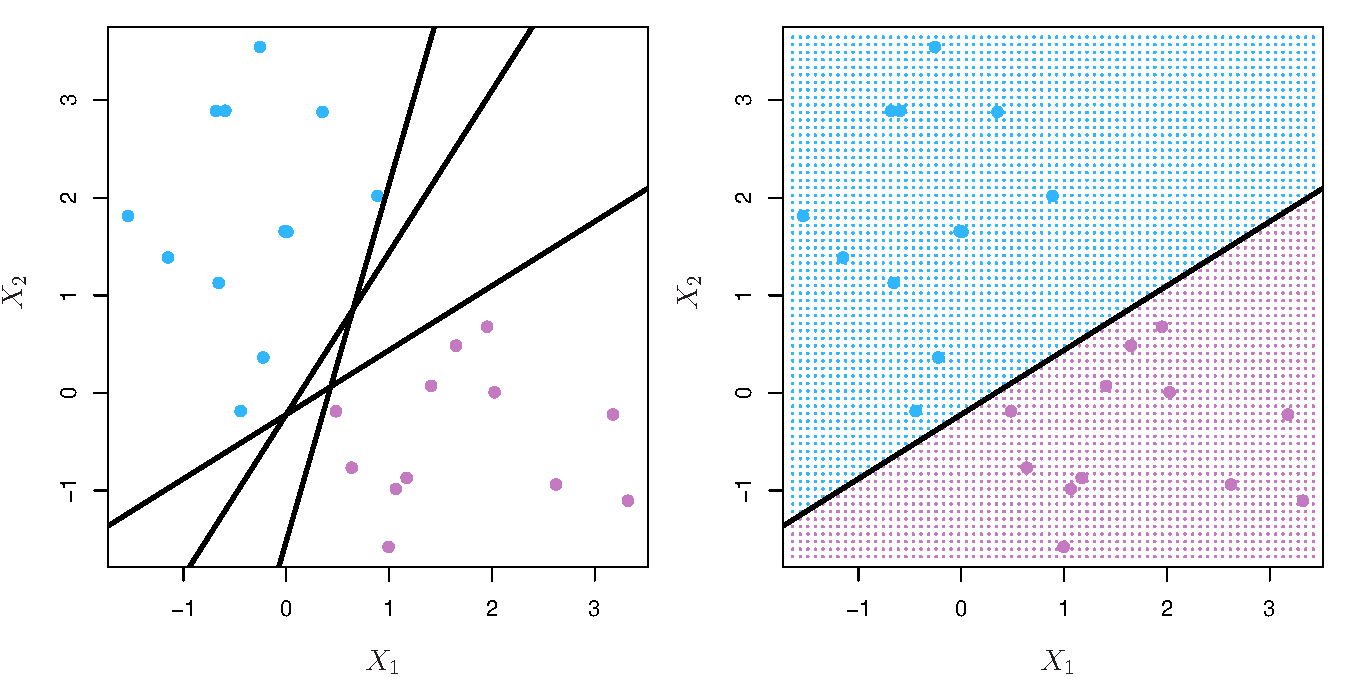
\includegraphics[width=12cm]{graphics/9_2.pdf}
  \caption{Left: Three possible hyperplanes for dividing two classes of observations. Right: A hyperplane separating two classes and grid illustrating which class observations would be assigned.\cite{jamesSupportVectorMachines}}
\end{figure}

\begin{figure}[ht]
  \centering
  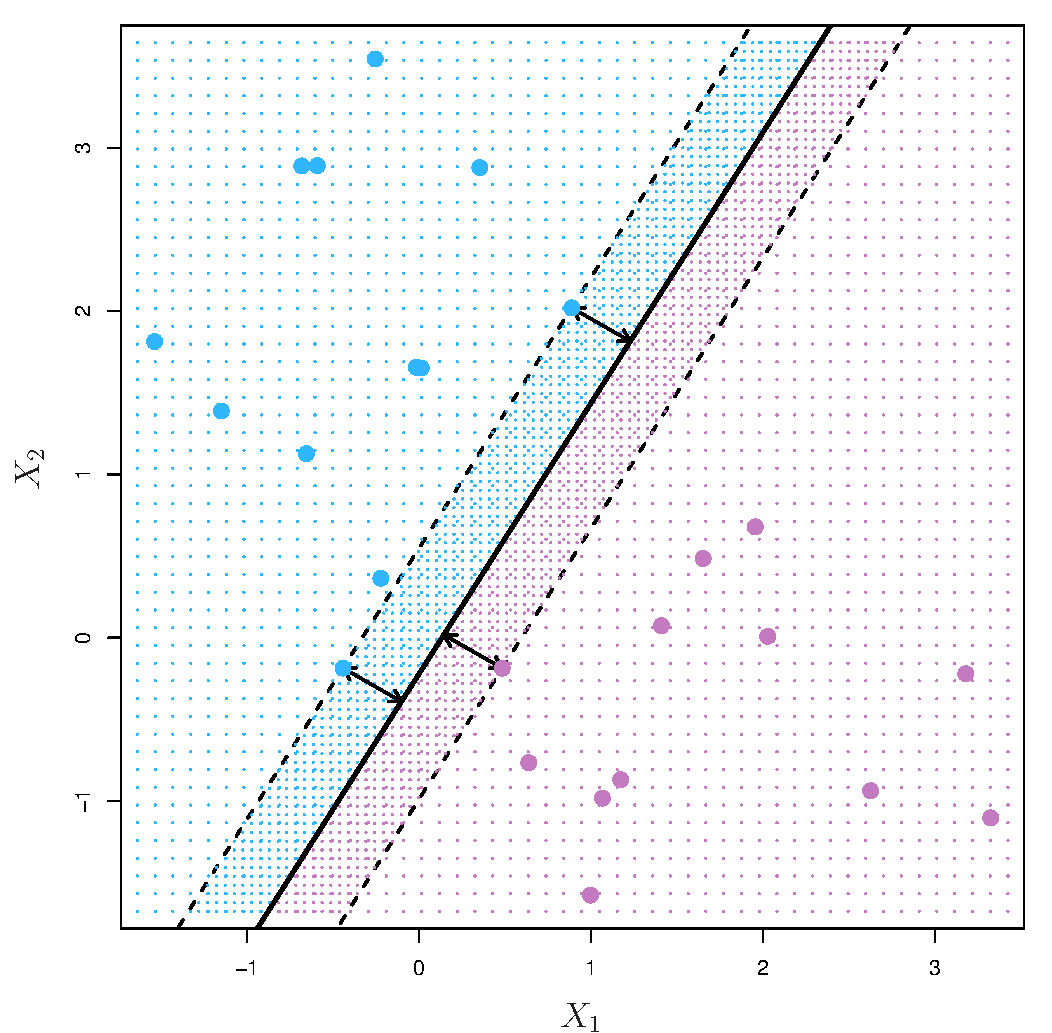
\includegraphics[width=12cm]{graphics/9_3.pdf}
  \caption{A maximal margin hyperplane, shown as a solid line, and the margin which is the distance between the solid and dashed lines.\cite{jamesSupportVectorMachines}}
\end{figure}

\begin{figure}[ht]
  \centering
  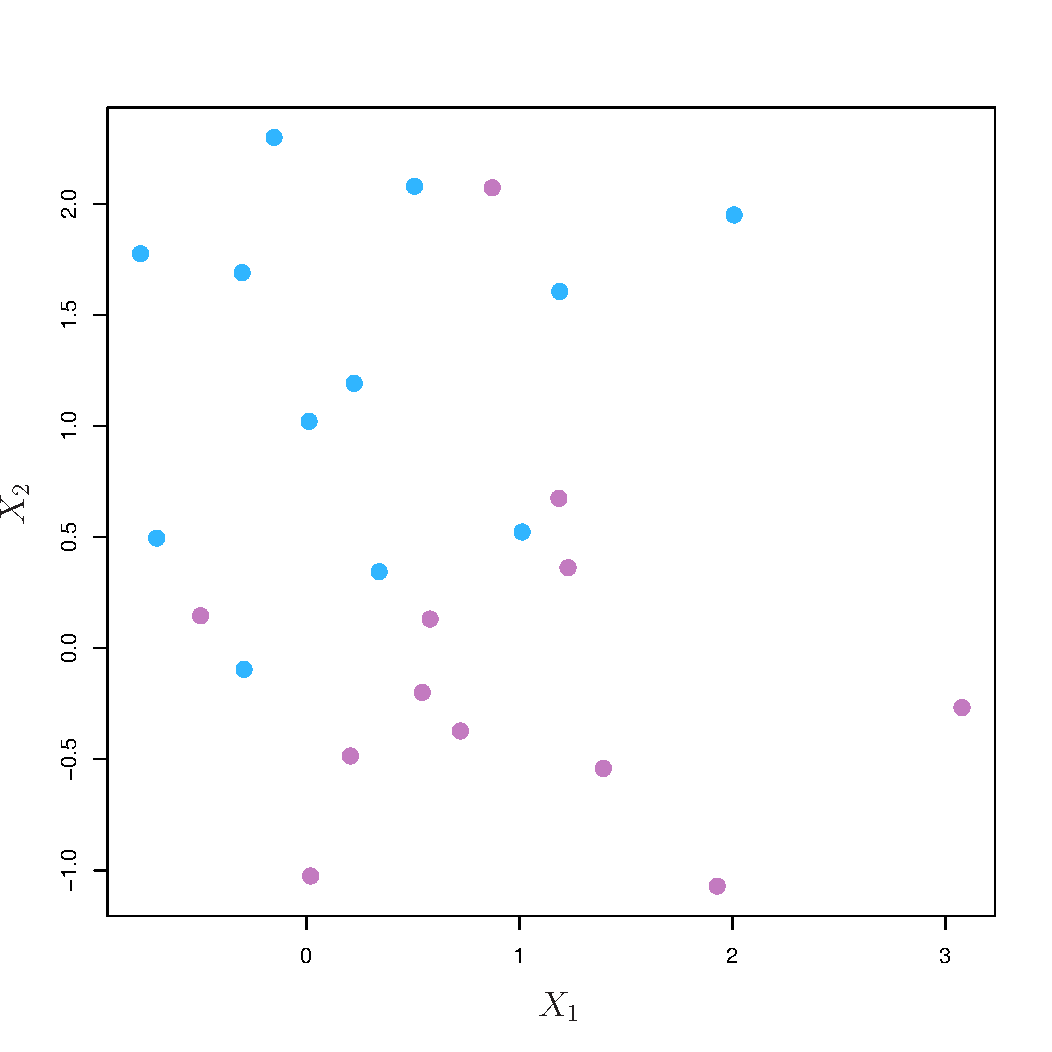
\includegraphics[width=12cm]{graphics/9_4.pdf}
  \caption{Two classes of observations that are not separable by a hyperlane, meaning that a \gls{mmc} cannot be used\cite{jamesSupportVectorMachines}}
\end{figure}

\begin{figure}[ht]
  \centering
  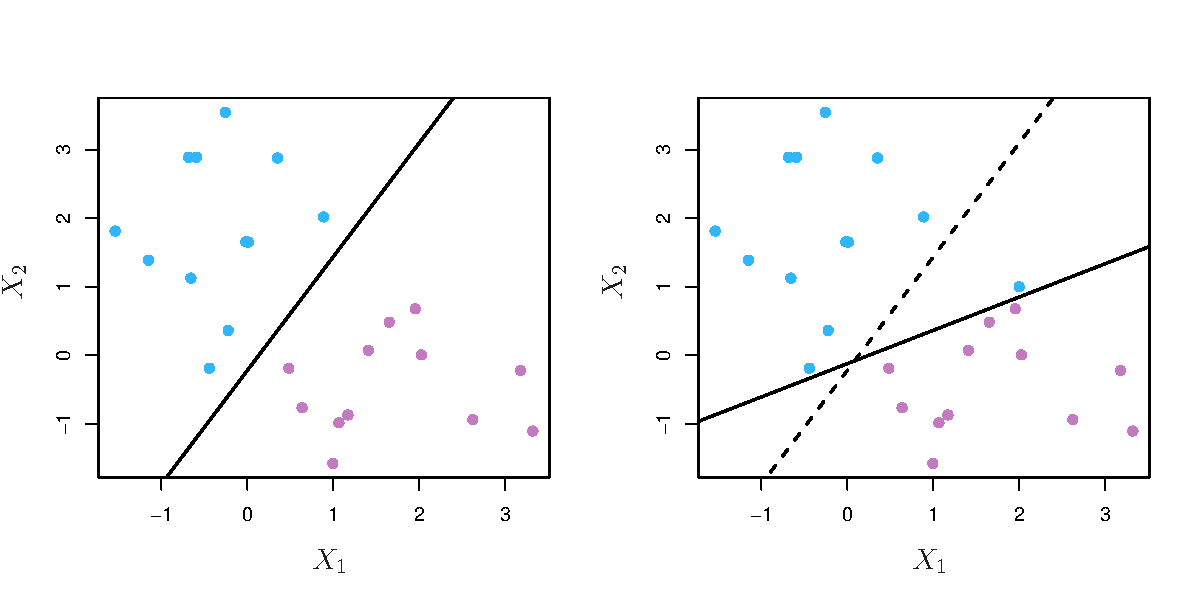
\includegraphics[width=12cm]{graphics/9_5.pdf}
  \caption{Left: Two classes separated by a maximal margin hyperplane. Right: A new maximal margin hyperplane (solid line) and the old maximal margin hyperplane (dashed line) illustrating the effect a single observation can have when using the \gls{mmc}.\cite{jamesSupportVectorMachines}}
\end{figure}

\subsubsection{Support Vector Classifier}
The \gls{svc}, also called the \textit{soft margin classifier}, is based on the \gls{mmc} but instead of making a hard margin it has a "soft" margin. This means that the \gls{svc} may allow some of the training observations to not only violate the margin but also the separating hyperplane in order to classify \textit{most} of the training data better. The soft margin of the \gls{svc} allows the classification of data that are not strictly separable by a hyperplane. It also means that a single observation in the training data has less impact on the separating hyperplane, which in some cases may cause an \gls{mmc} to make a less accurate classification for the majority of data.\cite{jamesSupportVectorMachines}

\begin{figure}[ht]
  \centering
  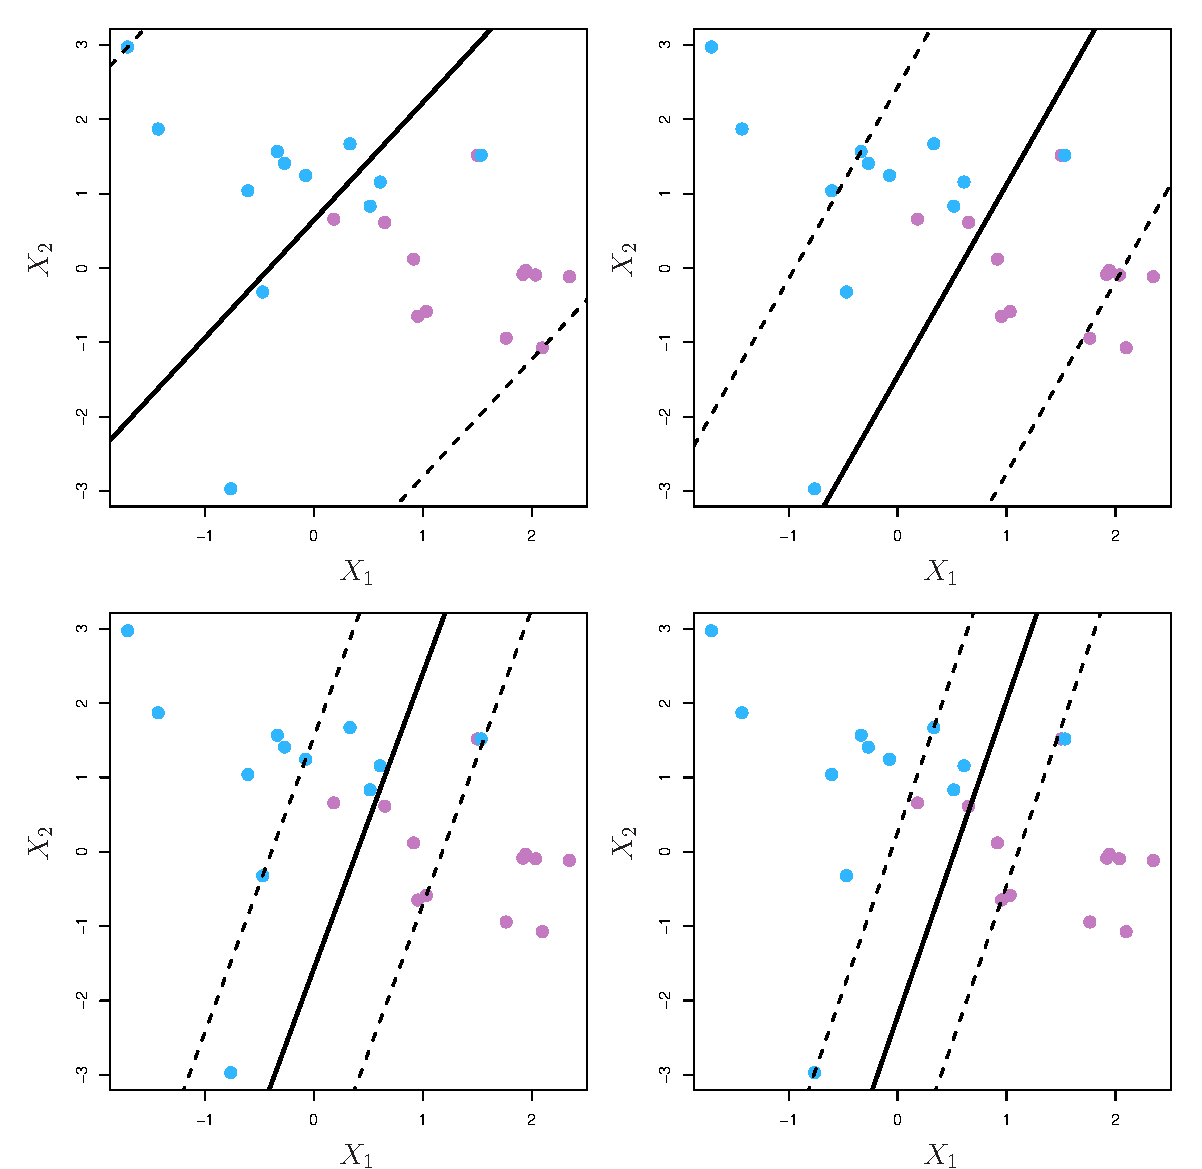
\includegraphics[width=12cm]{graphics/9_7.pdf}
  \caption{A \gls{svc} used for classifying data. In each case the tolerance of observations being on the wrong side of the margin and hyperplane is different, resulting in different classifying hyperplanes.\cite{jamesSupportVectorMachines}}
\end{figure}

\subsubsection{Support Vector Machine}
The \gls{svm} is and extension to the \gls{svc} with the use of kernels. The \gls{svm} enlarges the feature space in order to make non-linear division boundaries possible between classes, which the \gls{svc} cannot do as shown in figure 9. The type of kernel used with a \gls{svm}\cite{KernelMethod2021} determines what kind of function is used for the separation of classes\cite{SVMKernelsScikitlearn24}.\cite{jamesSupportVectorMachines}

\begin{figure}[ht]
  \centering
  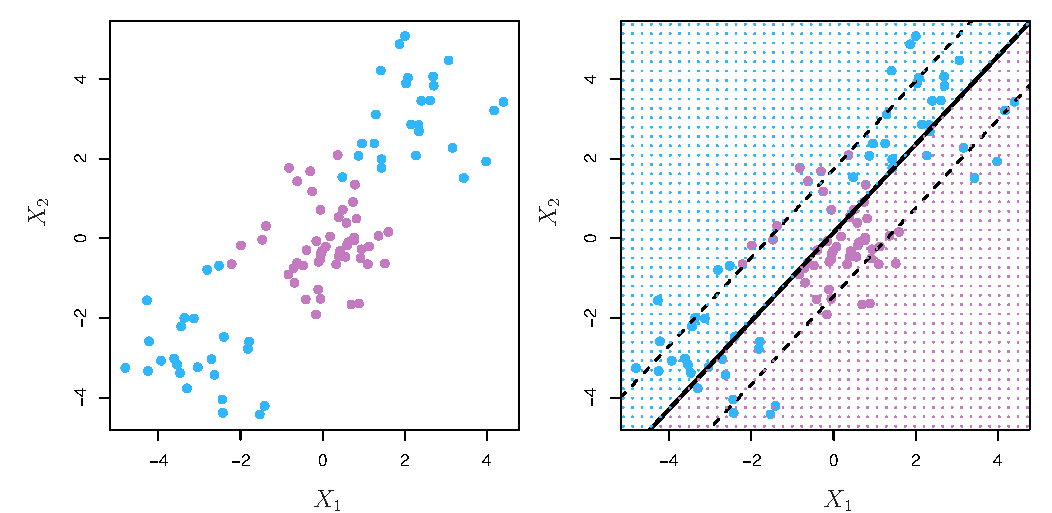
\includegraphics[width=12cm]{graphics/9_8.pdf}
  \caption{Left: Observations of two classes not divisible by a linear boundary. Right: The \gls{svc} trying to find a linear boundary between the two classes.\cite{jamesSupportVectorMachines}}
\end{figure}

\begin{figure}[ht]
  \centering
  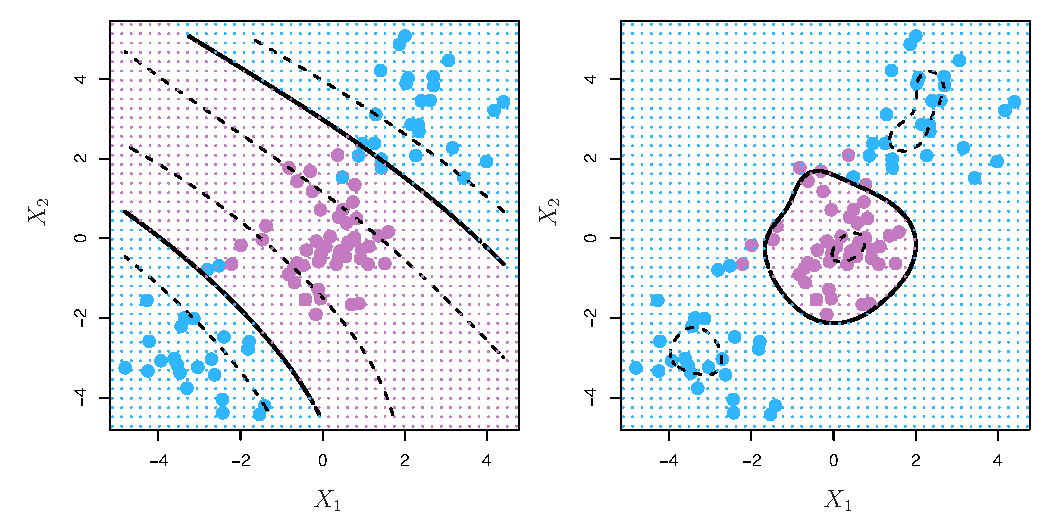
\includegraphics[width=12cm]{graphics/9_9.pdf}
  \caption{Left: A \gls{svm} with a polynomial kernel applied to non-linear data. Right: A \gls{svm} with a \gls{rbf} kernel applied to non-linear data.\cite{jamesSupportVectorMachines}}
\end{figure}

\subsubsection{SVMs with More than two Classes}
\glspl{svm} are in themselves not capable of separating more than two classes which necessitates the use of a way to extend \glspl{svm} to K-cases. The two most used and well-known methods are the \textit{one-versus-one} and \textit{one-versus-all}. In the case of this study the \textit{one-versus-one} approach is used for multi-class classifications\cite{jamesSupportVectorMachines}.\\
\\
\textbf{\textit{One-Versus-one Classification}}\\
The \textit{one-versus-one} approach for multi-class classification constructs $\binom{K}{2}$ \glspl{svm}, where each \gls{svm} compares two classes with each other. Thus each class is compared to all other classes individually.\cite{jamesSupportVectorMachines}\\
\\
\textbf{\textit{One-Versus-all Classification}}
Using the \textit{one-versus-all} method, for K $>$ 2, fits K \glspl{svm}. Each \gls{svm} is then compared to the remaining K - 1 classes.\cite{jamesSupportVectorMachines}

\subsection{Marshall \gls{ct} Score}
The Marshall classification of traumatic brain injury, or Marshall \gls{ct} score, is a metric used for classification of traumatic brain injury. The classification system is a \gls{ct} scan derived metric that has shown to predict patient outcome in cases of traumatic brain injury.\cite{gaillardMarshallClassificationTraumatic}\\
\\
The Marshall system divides patients into six categories.
Patients are divided into six categories (I to VI) by the Marshall system. Categorization is done on the basis of a non-contrast \gls{ct} scan of the brain. The severity increases with the numbers, VI being the most severe, and thus the higher numbers have worse prognosis and survival. The system focuses mostly on two features: Degree of swelling, which is determined by midline shift and/or compression of basal cisterns, and the presence and size of contusions/hemorrhages that are referred to as ``high or mixed density lesions'' in the classification.\cite{gaillardMarshallClassificationTraumatic}\\
\\
The scored elements in the Marshall classification are:

\begin{itemize}
\item{degree of basal cistern compression}
\item{degree of midline shift}
\item{presence and size of contusions/heemorrhages}
\end{itemize}

The classifications of the Marshall \gls{ct} score are the following:

\begin{enumerate}
\item{Diffuse Injury I}
  \begin{itemize}
    \item{no visible intracranial pathology}
  \end{itemize}
\item{Diffuse Injury II}
  \begin{itemize}
   \item{midline shift 0 to 5mm}
    \item{basal cisterns remain visible}
    \item{no high  or mixed density lesions $>25 cm^3$}
  \end{itemize}
\item{Diffuse Injury III}
  \begin{itemize}
    \item{midline shift 0 to 5mm}
    \item{basal cisterns compressed or completely effaced}
    \item{no high or mixed density lesions $>25cm^3$}
  \end{itemize}
\item{Diffuse Injury IV}
  \begin{itemize}
    \item{midline shift $>5 mm$}
    \item{no high or mixed density lesions $>25cm^3$}
  \end{itemize}
\item{Diffuse Injury V}
  \begin{itemize}
    \item{any lesion evacuated surgically}
  \end{itemize}
\item{Diffuse Injury VI}
  \begin{itemize}
    \item{high or mixed density lesions $>25cm^3$}
    \item{not surgically evacuated}
  \end{itemize}
\end{enumerate}

\subsection{Rotterdam \gls{ct} Score}
The Rotterdam \gls{ct} score of traumatic brain injury is a classification purposed for improving prognostic evaluation for patients admitted with acute traumatic brain injuries. The Rotterdam system is more recent than the Marshall classification of traumatic brain injury which tries to address some of the limitations that the older Marshall system has. Instead of having three independently scored elements the Rotterdam system has four, and one of the elements is slightly different from the Marshall system.\\
\\
The scored elements in the Rotterdam classification are:

\begin{itemize}
\item{degree of basal cistern compression}
\item{degree of midline shift}
\item{epidural hematomas}
\item{intraventricular and/or subarachnoid blood}
\end{itemize}

The classification of the Rotterdam \gls{ct} score is scored by the following system:

\begin{itemize}
\item{basal cisterns}
  \begin{itemize}
    \item{0: normal}
    \item{1: compressed}
    \item{2: absent}
  \end{itemize}
\item{midline shift}
  \begin{itemize}
    \item{0: no shift or $\geq$ 5mm}
    \item{1: shift $>$ 5mm}
  \end{itemize}
\item{epidural mass lesion}
  \begin{itemize}
    \item{0: present}
    \item{1: absent}
  \end{itemize}
\item{intraventricular blood or \gls{tsah}}
  \begin{itemize}
    \item{0: absent}
    \item{1: present}
  \end{itemize}
\end{itemize}
The final score is the sum of the scores for each individually assessed element + 1.\\
\\
The Rotterdam \gls{ct} score has probability of mortality at six months post-injury for each score.\\
\begin{enumerate}
  \item{0\%}
  \item{7\%}
  \item{16\%}
  \item{26\%}
  \item{53\%}
  \item{61\%}
\end{enumerate}

\subsection{Extended Glasgow Outcome Scale}
The GOS-E, or \gls{gose}, is an extension developed to the original Glasgow outcome scale (GOS) in 1981 to address some of its limitations. The original GOS has five categories, these are extended to eight in the GOS-E. In 1998 a questionnaire with guidelines was provided to improve the reliability of the GOS ans GOS-E ratings\cite{GOSEExtendedGlasgow}.\cite{sanderExtendedGlasgowOutcome2002}\\
\\
The categories of the GOS-E are:
\begin{itemize}
  \item{Dead}
  \item{Vegetative State}
  \item{Lower Severe Disability}
  \item{Upper Severe Disability}
  \item{Lower Moderate Disability}
  \item{Upper Moderate Disability}
  \item{Lower Good Recovery}
  \item{Upper Good Recovery}
\end{itemize}

\subsection{Patient Injuries}

\subsubsection{\gls{ct} Brain Pathology}
Brain pathology is disease in the brain, \gls{ct} brain pathology is the study of brain diseases which can be found by a \gls{ct} scan.
The data indicates whether any brain pathology could be indicated via a \gls{ct} scan.\cite{BrainPathologyDefinition}

\subsubsection{\gls{ct} Skull Fracture}
The cranial portion of the skull consists of eight bones. A skull fracture is a fracture or break in any one of these bones. A skull fracture may cause underlying structures such as membranes, blood vessels and brain to be damaged.\cite{SkullFracture2020}\\
\\
If no part of skull bone causes damage to tissue around it a skull fracture in itself is not that significant. Skull fractures can occur without there being any other physical or neurological damage. It is however indicative of a significant amount of force applied to the head if there is a skull fracture in healthy bone. When a skull fracture is caused to healthy bone it is likely that this person has suffered a concussion, whether with or without loss of consciousness.\cite{SkullFracture2020}

\subsubsection{\gls{ct} Skull Base Fracture}
Skull base fractures, often referred to as basal or basilar skull fractures, is the break of a bone in the base of the skull. The bones the break can occur in are the temporal bone, occipital bone, sphenoid bone, frontal bone, or ethmoid bone. Depending on where the fracture has occurred the fractures are divided into anterior, central or posterior fractures. For a skull base fracture to occur it generally requires a significant amount of trauma. The diagnosis of basal skull fractures is mostly done by a \gls{ct} scan.\cite{BasilarSkullFracture2021}\\
\\
Symptoms that can be caused by basal skull fractures include bruising behind the ears, bruising around the eyes, blood behind the ear drum, and \gls{csf} leak, which occurs in about 20\% of cases, that may cause fluid to leak from nose or ears. Other possible effects are cranial nerve or blood vessel injury and about 14\% of cases cause in meningitis, which is the inflammation of the protective membranes that cover the brain and spinal chord.\cite{BasilarSkullFracture2021}\\
\\
\begin{figure}[ht]
  \centering
  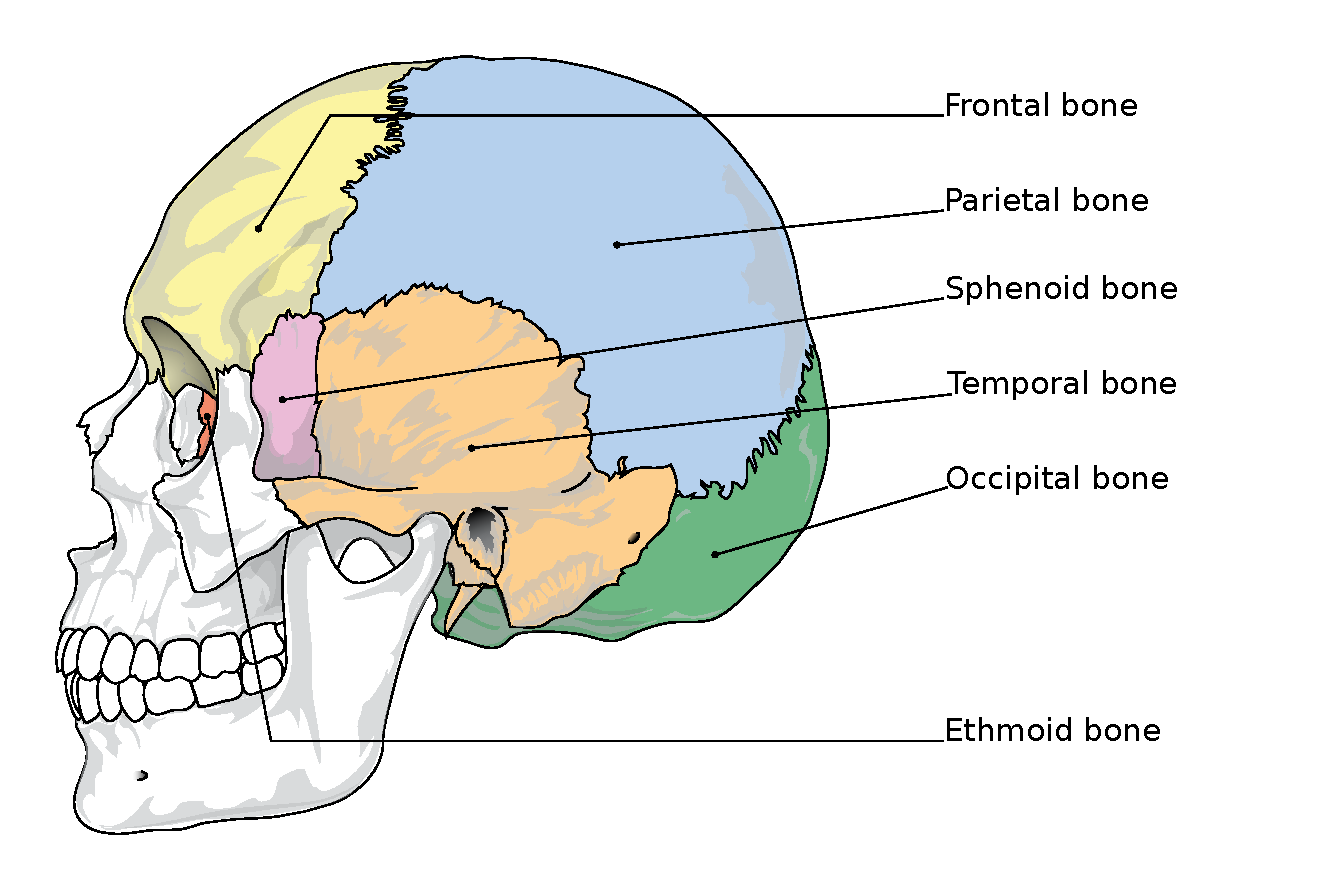
\includegraphics[width=12cm]{graphics/cranial_bones.pdf}
  \caption{Figure showing what bones may be involved in a basal skull fracture\cite{BasilarSkullFracture2021}}
\end{figure}

\subsubsection{Facial Fracture}
Facial fractures are fractures caused to a facial bone and are most commonly caused by blunt or penetrating trauma\cite{ibrahimFacialFracturesRadiology}. As some of the facial bones are close to the brain, fractures in those bones may cause complications in the brain and \gls{cns}.\cite{FacialFracturesTypes}

\subsubsection{Epidural Hematoma}
An epidural hematoma is a bleed between the \gls{dm} and the skull, typically caused by an injury that causes a break in the temporal bone and bleeding from the \gls{mma}, but also sometimes caused by bleeding disorders or malformation of blood vessels. Symptoms that may be cause by an epidural hematoma include headaches, confusion, vomiting, inability to move some body parts and seizures. Epidural hematomas occur in about 1-4\% of head injuries and 15\% of fatal head injuries. Epidural hematomas are generally treated by surgery. If an epidural hematoma is left untreated it usually results in death.\cite{EpiduralHematoma2021}\\
\\
When receiving an injury that causes an epidural hematoma it is often followed by a loss of consciousness, then a short regaining of consciousness, and then loss of consciousness again. If this lucid period occurs the prognosis for the patient is better than if the patient does not regain consciousness. If the hematoma is arterial the progress is usually rapid and if venous it is slower. The size of the hematoma at the time of surgery also effects the outcome.\cite{EpiduralHematoma2021}

\subsubsection{Subdural Hematoma}
\glspl{sh} are a bleeding where blood collects between the \gls{dm} and \gls{am} that surround the brain. Generally it is the results from tears in \gls{bv}. \gls{sh}s can cause the pressure in the skull to increase which can cause damage to brain tissue.\cite{SubduralHematoma2021}\\
\\
Chronic \glspl{sh} are bleedings that slowly increase the size of the hematoma with recurret bleeding that may be caused by a variety of complications\cite{yadavChronicSubduralHematoma2016}. Chronic \glspl{sh} have a better prognosis than acute \glspl{sh} if they are treated. Chronic \glspl{sh} can however be hard to detect as the symptoms are not alway clear, especially with older patients where other causes for their symptoms may be suspected\cite{yadavChronicSubduralHematoma2016}.\cite{SubduralHematoma2021}\\
\\
Acute \gls{sh} is generally life threatening as it puts pressure on blood vessels that supply the brain with blood so that the brain is not supplied with enough blood. This can then lead to death of brain cells. The subdural hematoma grows larger because as the intracranial pressure increases blood is pushed into the \glspl{dvs} which causes the dural venous pressure to rise increasing the bleeding from the ruptured \glspl{bv}. Only when the pressure of the hematoma and the intracranial pressure become equal does the growth of the \gls{sh} stop.\cite{SubduralHematoma2021}

\subsubsection{Subarachnoid Hemorrhage}
\gls{sah} is the bleeding into the \gls{susp}. \gls{sah} often occurs as the result of a head injury but can also occur spontaneously from a \gls{ca} that has ruptured. Symptoms caused by \gls{sah} may include severe headaches, vomiting, decreased consciousness levels, fever, seizures, neck pain and/or stiffness.\cite{SubarachnoidHemorrhage2021}\\
\\
Spontaneous \gls{sah} affects about one per 10 000 people per year. Many underlying health factors affect the prominence of spontaneous \gls{sah} and it becomes more common with age. About half of the people with \gls{sah} due to an aneurysm die within 30 days of the hemoorhage and a third of those who survive have problems later in life as the result of the \gls{sah}.\cite{SubarachnoidHemorrhage2021}\\
\\
\Gls{tsah} is a common injury that occurs in about 11-60\% of \gls{tbi} cases\cite{knipeTraumaticSubarachnoidHemorrhage}. \gls{tsah} however has a much lower mortality rate that spontaneous \gls{sah} and only about 10\% have worsening of head injuries following a \gls{tsah}\cite{cooperManagementTraumaticSubarachnoid2019}. As \gls{tsah} is quite common in cases of \gls{tbi} it often occurs in addition to other forms of brain injury. In these cases the prognosis is worse but it is not clear if this is a result of the \gls{sah} or if it just indicates a more severe brain injury.\cite{SubarachnoidHemorrhage2021}\\
\\
The long term effects of \gls{sah} are common. Long term symptoms may include fatigue and mood disturbances. Even for those that have made a good neurological recovery anxiety, depression, \gls{ptsd}, and cognitive impairments. In total about 46\% of those that have suffered a \gls{sah} get cognitive impairments that effect their quality of life.\cite{SubarachnoidHemorrhage2021}

\subsubsection{Contusion}
Cerebral contusions are a bruise of the brain tissue, and like other bruises are many microhemorrhages, that leak blood into the brain tissue. Cerebral contusions occur in 20-30\% of severe cases head injury but often heal on their own without any medical intervention. Cerebral contusions can however cause lowered mental function in the long term and in short term may cause \gls{bh}, a life threatening condition which requires prompt measures to be taken\cite{BrainHerniation2020}.\cite{CerebralContusion2020}

\subsubsection{Midline Shift}
Midline shift is when the brain is moved from its center line. The finding of midline shift implies the risk of distortion of the brain stem which can cause serious harm. Midline shift is also commonly associated with high \gls{icp} which can be fatal, as it can cause crushing of brain tissue, shifts in brain structures, restrict blood supply to the brain, cause \gls{bh} and contribute to \gls{hc}\cite{IntracranialPressure2021}.\cite{MidlineShift2021}

\begin{figure}[ht]
  \centering
  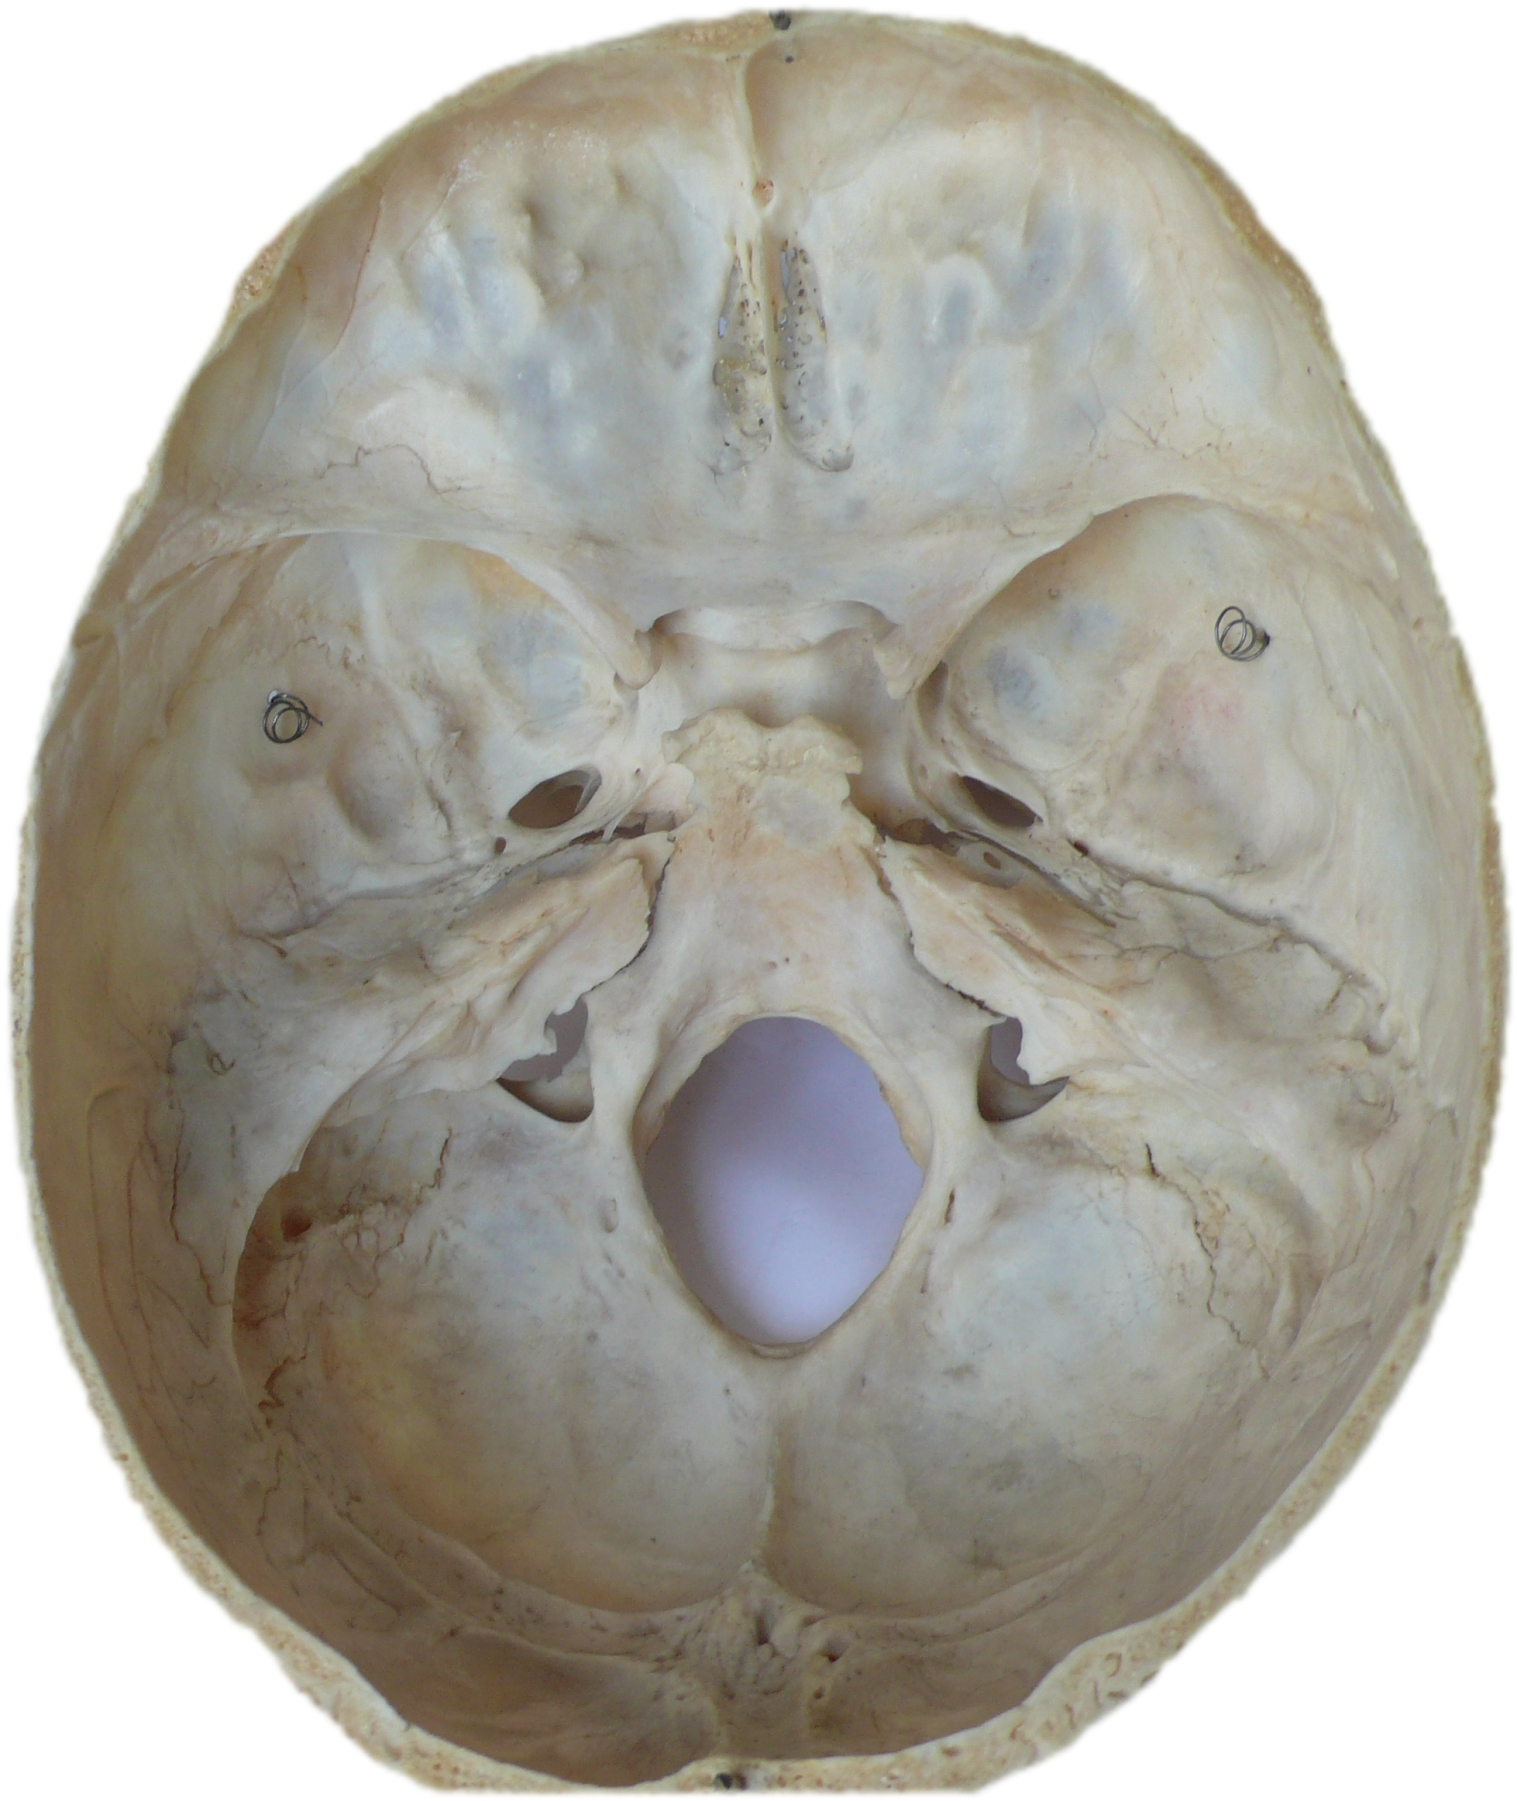
\includegraphics[width=10cm]{graphics/skull_interior.jpeg}
  \caption{The inside of the skull. There are many ridges which can cause injuries to the bran if it moves along them.\cite{CerebralContusion2020}}
\end{figure}

\subsubsection{Cisternal Compression}
Cisternal compression refers to the compression or absence of \glspl{bc}, also called subarachnoid cisterns or cerebral cisterns. There has been shown to be a strong relation between patient outcome and the state of the \glspl{bc} with those having compressed basal cisterns having higher mortality rates than those with normal \glspl{bc} and even higher mortality rates for those with absent \glspl{bc}\cite{toutantAbsentCompressedBasal1984}\cite{kouvarellisRelationshipBasalCisterns2011}. Absence of \glspl{bc} meaning them having being obliterated\cite{kouvarellisRelationshipBasalCisterns2011}.

\subsection{Patient Genetics}

\subsubsection{rs4680}
rs4680, sometimes also referred to as Val158Met, Val108/158Met or G1947A, is a \gls{snp} in the \gls{comt} gene. The nucleotide substitution between A and G results in changing the amino acid at codon 158 from valine, for genotype G;G, to methionine, for genotype A;A. The A/Met allele makes a change in the enzyme which has been shown to have lower enzymatic activity (because of thermoinstability).\cite{Rs46802020}\\
\\
The activity is supposedly only 25\% of the enzyme coded for in the case of the G/Val allele\cite{Rs4680SNPedia}. This change in the activity of the enzyme may influence the outcome following severe head trauma and have been show to have an association in outcome following mild \gls{tbi}.\cite{winklerCOMTVal1582016}

\subsubsection{rs6277}
rs6277 (957C$>$T, Pro319Pro) is an \gls{snp} in the \gls{drd2} gene\cite{Rs6277SNPedia}. It has been shown that there could be a significant association between susceptibility to PTSD and the rs6277 \gls{snp} with individuals having PTSD being more likely to carry the C allele\cite{voiseyDRD2Gene957C2009}.
\subsubsection{rs3219119}
The rs3219119 \gls{snp} has been shown to potentially be an indicator for the outcome in \gls{tbi} cases. It is however not the rs3219119 alone that impacts the outcome in \gls{tbi} as the \gls{snp} is closely associated with the rs3219090 \gls{snp} and the effects caused by variations in one are not independent from variations in the other.\cite{sarnaikInfluencePARP1Polymorphisms2010}

\subsubsection{rs11604671}
rs11604671 is a \gls{snp} in the \gls{ankk1} gene\cite{Rs11604671SNPedia}. Variations in the \gls{snp} have been shown to along with the \glspl{snp} rs4938016 and rs1800497 to have an impact on cognitive outcome measures after \gls{tbi}.\cite{mcallisterSingleNucleotidePolymorphisms2008a}

\subsubsection{rs4938016}
rs4938016 is a \gls{snp} in the \gls{ankk1} gene\cite{mcallisterSingleNucleotidePolymorphisms2008a}. Variations in the \gls{snp} have been shown to along with the \glspl{snp} rs11604671 and rs1800497 to have an impact on cognitive outcome measures after \gls{tbi}.\cite{mcallisterSingleNucleotidePolymorphisms2008a}

\subsubsection{rs1800497}
rs1800497 is a \gls{snp} in the \gls{drd2} gene\cite{Rs1800497SNPedia}. Variations in the \gls{snp} have been shown to along with the \glspl{snp} rs3219119 and rs4938016 to have an impact on cognitive outcome measures after \gls{tbi}.\cite{mcallisterSingleNucleotidePolymorphisms2008a}

\section{Method}
The classifications were all performed in the Python programming language using the scikit-learn algorithm. The code for the program is found in the appendix.\\
\\
The program imports the data from an external file (can be found at: \href{https://data.world/deviramanan2016/traumatic-brain-injury}{TBI dataset})\cite{TraumaticBrainInjurya}, and as the data is not entirely complete any datapoints that are missing any data that is to be used are dropped. The data used for prediction and the data that is to be predicted are then put into separate variables (found in the appendix as "X" and "y" respectively). The data in both variables is the separated into training data, which is used to make the prediction model, and testing data, which is used to test the model's accuracy.\\
\\
The algorithm is then run using the test and training data after which its accuracy metric is evaluated. The support vector machine is a supervised learning method which means the data has to be split up into training and testing data. This split affects the results when the classification is scored. Using different training data means the classes will be different and thus it will classify the data differently depending on the training data. For this reason the accuracy of the function varies, so 3000 iterations have been run for all the results after which the average score is given. This ensures that the result of a single iteration of the algorithm has little impact on the total results.\\
\\
When running the algorithm the desired parameters for the kernel and class weight are set, and in the case of the polynomial kernel the degree of the polynomial is also set. For each prediction the algorithm was run with the linear, radial basis function, and polynomial kernel (with degree=3). For each of the kernels the algorithm was also run both with a class wight that was balanced and one that was not.\\
\\
The prediction of the Marshall and Rotterdam \gls{ct} scores (found under the section "Background") were made using the patient injuries (found under "Patient Injuries" in the section "Background"). The prediction of the \gls{gose} and \gls{ptsd} scores were made first using the Marshall and Rotterdam \gls{ct} scores alone and then along with the patients genetic factors (found under "Patient Genetics" in the section "Background").


\section{Results}

\subsection{Prediction of Marshall and Rotterdam \gls{ct} scores}
Using patient injuries for predicting their Marshall and Rotterdam \gls{ct} scores.\\
\begin{center}
  Left: Classification of Marshall score. Right: Classification of Rotterdam score.
  \csvautotabular{result/svm_inj_mar.csv} \hspace{.5cm}
  \csvautotabular{result/svm_inj_rot.csv}
\end{center}

\subsection{Prediction of \gls{gose} and \gls{ptsd}}
Using the Marshall and Rotterdam \gls{ct} scores for predicting GOS-E score and PTSD 6 months after injury.\\
\begin{center}
  Left: Classification of 6 month GOS-E. Right: Classification of 6 month PTSD.\\
  \csvautotabular{result/svm_mar_rot_gose6m.csv} \hspace{.5cm}
  \csvautotabular{result/svm_mar_rot_ptsd.csv}
\end{center}
\vspace{1cm}
Using the Marshall and Rotterdam \gls{ct} scores along with the genetic factors for predicting GOS-E score and PTSD 6 months after injury.\\
\begin{center}
  Left: Classification of 6 month GOS-E. Right: Classification of 6 month PTSD.\\
  \csvautotabular{result/svm_comb_gose6m.csv} \hspace{.5cm}
  \csvautotabular{result/svm_comb_ptsd.csv}
\end{center}
For classification of \gls{ptsd} both when using only the Marshall and Rotterdam \gls{ct} scores alone and when using them along with the genetic factors the algorithms that were run with class weight one classified all datapoints as not having \gls{ptsd} after six months. For classification of \gls{gose} using the Marshall and Rotterdam \gls{ct} score, the linear kernel, and class weight one the algorithm only classified the \gls{gose} score as 1, 6 or 8.

\section{Conclusions}

\begin{enumerate}
  \item{The Marshall \gls{ct} score can be predicted with high accuracy with a SVM using injuries (see listed) as factors}
  \item{The Rotterdam \gls{ct} score can be predicted with moderately high accuracy with a SVM using injuries (see listed) as factors}
  \item{The 6 month GOS-E score is not reliably predicted with a SVM using the Rotterdam and Marshall \gls{ct} sores as factors}
  \item{The 6 month PTSD is not reliably predicted with a SVM using the Rotterdam and Marshall \gls{ct} scores as factors}
  \item{The 6 month GOS-E score is not reliably predicted with a SVM using both genetics and the Rotterdam and Marshall \gls{ct} scores as factors}
  \item{The 6 month PTSD is not reliably predicted with a SVM using both genetics and the Rotterdam and Marshall \gls{ct} scores as factors}
\end{enumerate}
\section{Discussion}

\subsection{Classification of 6 month \gls{ptsd} and \gls{gose}}
As can clearly be concluded from the results, the \gls{svm} could not reliably make predictions for the long term effects that patients had based on the Rotterdam and Marshall CT scores. Neither did it make any substantial difference if genetic factors for the patients were included along with the Rotterdam and Marshall CT scores. This is not altogether surprising as the brain is such a complex organ and the Rotterdam and Marshall CT scores are a relatively simple patient outcome and mortality prognosis. Similarly genetics, even though they may make some difference in cases of brain injury, rarely depend on just a few genetic differences. Additionally genetic differences are likely to have a lesser impact on patient outcome than the injuries a person has sustained, as such the genetic differences between patients are not likely to help in the prediction of outcome if there is not already a relatively accurate way of doing this without any genetic factors.\\
\\
The classification for both six month \gls{ptsd} and \gls{gose} were made using the Marshall and Rotterdam CT scores. This means that the data is already interpreted by humans before the \gls{svm} uses the data. This causes problems as is discussed under the subsection "Method" and as such are not optimal for predicting the patient outcome. What can be done is to determine how well these systems for prognosis created by humans work for predicting the long term outcome for patients and how well they translate into predicting other metrics than what they were explicitly designed for.

\subsection{Classification of Marshall and Rotterdam \gls{ct} scores}
For the predicion of the Rotterdam CT score and the Marshall CT score using patient injuries as factors the accuracy of prediction was considerably higher than for the 6 month \gls{ptsd} and \gls{gose}. This can be expected as the scores are defined by presence and degree of injuries which are present in the data. The degree of these injuries is however not present and the predictions were made along with several other injuries that are not accounted for when determining the Marshall and Rotterdam CT scores. As such it would be expected that if one were to run the algorithm using only the injuries which determine the Marshall CT score and Rotterdam CT score along with the degree of said injuries the predictions would be 100\% accurate, however in that case one might as well just determine the score using the set rules for the scores.\\
\\
Classifying the Marshall score the \gls{svm} has an average accuracy between 86 and 88\%. This score can be considered high enough to give information of a patients Marshall score with some confidence. Classifying the Rotterdam CT score the \gls{svm} has an average accuracy between 71 and 77\%, which is considerably lower than for the Marshall CT score. This level of accuracy can be considered to give some indication of a patients Rotterdam score however the likelihood of it being wrong is also relatively high.\\
\\
What is interesting is the fact that data for other injuries does not disrupt the accuracy for the prediction of the Rotterdam and Marshall CT scores so that the predictions would become inconstitent. And as the accuracy is about the same both when the class weight is the same for all factors and when they are balanced it indicates that the predictions do not rely solely on the factors which define the scores. This could indicate that the Marshall and Rotterdam CT scores do in some way reflect the total degree of damage that a patient has suffered. However to know if this were the case more specific research would have to be conducted on that exact question. The results also show a difference between the Marshall and Rotterdam CT scores as the prediction accuracy for the Marshall CT score was consistently 10-15 percentage points higher than that for the Rotterdam CT score. This indicates that the Marshall CT score is better represented by the injuries which were used to predict the score.\\
\\
The fact that the score is rather high is not that surprising considering how the Marshall \gls{ct} score is determined. It is determined using midline shift and/or the compression of basal cisterns, and the presence and size of contusions or hemorrhages. A lot of this information is also given to the SVM in the dataset which means the algorithm uses the data of the same injuries to determine the Marshall score as is used by humans to set the score. There is one difference though, which is that the data used for training the SVM has no information on the degree of midline shift or the degree of basal cistern compressions. The data only contains if a patient has midline shift or not and if it has basal cistern compressions or not.\\
\\
Even though the SVM scores quite high in classifying the Marshall \gls{ct} score it is less accurate for the higher scores. This is likely due to the fact that the dataset is quite small and that the amount of patients with more severe \gls{tbi} is even smaller. This makes it harder to make clear boundaries for the SVM. Another thing that might affect the accuracy of higher scores is the fact that those are more reliant on the degree of the different injuries used for classification and not merely if the injury has been observed or not.\\
\\
It is likely however that even if the higher scores rely more on the degree of injuries the accuracy might be noticeably higher if the dataset used would be larger.

\subsection{Injury Factors}
One of the major restrictions created by the data is the fact that a lot of the specifics for injuries are left out. Mostly the data just indicates if a particular injury was present or not. This makes it more difficult to predict outcome as there is no way of knowing to which extent this injury might have affected the patient. For example the data states whether or not a patient has suffered midline shift but not how great the shift was and if a patient had cisternal compressions but not if they were only compressed or had been completely eradicated. For both of these the degree of injury has major implications on patient outcome.\\
\\
Some of the data is also unclear to its extent. The data includes cerebral contusions but not cerebral lascerations. The distinction between which is that in the case of a cerebral lasceration the \gls{pm} and \gls{am} have been torn at the site of the injury but not in the case of cerebral contusions. As patients have been examined for cerebral contusions which is done by a CT scan\cite{CerebralContusion2020}, the same as cerebral lascerations\cite{CerebralLaceration2018}, the distinction between the injuries could have been made. However the two injuries are grouped together in some classification systems (ICD-9 \& ICD-10\cite{CerebralLaceration2018}\cite{ICD102021}) as they are quite similar.

\subsection{The classification choice problem \& correctness metrics}
For classification of \gls{tbi} it is intended to get a prediction of what class an injury is and how it affects the person in question. This leads to a problem that is: What are the classes? The purpose of this kind of algorithm would be to classify the patients into groups but the problem is defining a group.\\
\\
If the groups are pre-defined the algorithm will try to fit the predictions within the boundaries of these groups, which causes a problem as the data might not actually "fit" within these groups properly, instead it could be better to use other groups. Knowing what groups would be best to use can however be hard. One way of addressing the problem would be with trial and error to see which definition of classes is most suitable for the prediction model. Another way would be to first determine group boundaries for a dataset. This could be based on the distance between datapoints in an n-dimensional matrix. After the groups had been determined an analysis could be made of what traits the data in each group has. Both of these systems have some drawbacks and benefits. Pre-defined classes allows for the prediction of for this exact class which might be favorable, but as the data might not be suitable it could give worse accuracy. Defining classes for a specific dataset allows for "better" and more accurate classes, but it lacks the specificity that pre-defined classes can have, the results might be inconsistent if the dataset is not sufficiently large and varied and the classes might rely heavily on the exact factors that were used for the classification.\\
\\
When scoring the predictions made by any type of machine learning of artificial intelligence there are different metrics that can be used. In the case of this study only the accuracy measure is presented in the results. The accuracy is very simple, it shows the percentage of correct predictions for the test data, however it is not always indicative of how well the predictions have been made. Especially in cases such as this where the data is unbalanced, that is when a majority of the datapoints fall into a single or a few of many classes.\\
\\
The accuracy score for the prediction of \gls{ptsd} is 30-44\% when using balanced class wights and 75-76\% when class wights are all the same. When balancing class weight the algorithm overcompensates for the low amount of datapoints with \gls{ptsd} so that many are predicted to have \gls{ptsd} even though they do not, and if the class weight is not balanced all predictions are made as 0/false (predicting a patient will not have \gls{tbi}) and thus getting a high accuracy as about 75\% of the patients did not have \gls{ptsd} after six months. In this case the accuracy is quite high but the sensitivity/recall, that is the proportion of patients that had \gls{ptsd} and were predicted as such, is 0\%. The same principles also apply to the predictions of the Marshall and Rotterdam CT scores and six month \gls{gose} score as the data is also very unbalanced for these.\\
\\
If further analysis should be done to the results one might include precision, recall and specificity as correctness metrics.

\subsection{Method}
The dataset that is used has a quite limited sample size. The number of samples being so low means that there is a low chance of there being great consistency to be found in the data. What also affects the results is an inherent flaw in the way the research has been conducted. As the intention of a program like this is to find patterns where we humans cannot find them it is important that the program get raw data of it. In this case the data has already been processed by humans which means that the program only has access to data that has already been interpreted. If humans cannot, using their observations, with certainty say what has been damaged in the brain and what this will lead to the data that the humans collect will be flawed in this same way.\\
\\
To increase chances of success in a project like this it would be advised to use data that has in no way been interpreted by humans. Imaging of the brain is what would be most easily accessible and also seems to be the most relevant for this purpose. Then letting an  algorithm try to classify them into subgroups. Using data for which type of injuries a patient has suffered, although already interpreted by humans and classified by their definitions, could work if enough specifics would be included in the data. There is one advantage to this, which is that scientists have long studied how specific injuries affect humans. With this information it would be easier to manually optimize an algorithm for prediction of the effects caused by these injuries. Another alternative would be to use a neural network and feed it raw data that could be considered relevant to the prediction. A neural network could be more accurate and more reliable than a simpler manually optimized algorithm, however it would likely require a much larger quantity of data to train it to work properly. Sufficiently complex neural networks would also learn overtime as new data is given to them, which might make a better predictor with time.
\clearpage

\printglossary
\printglossary[type=\acronymtype]


\printbibliography
\clearpage

\section*{Appendix}

\begin{verbatim}

import numpy as np
import pandas as pd
import sklearn
from sklearn import svm
from sklearn import metrics

#loading data
data = pd.read_csv("data/journal_pone_0169490_s010.csv")

data = data[["gose_overallscore6m", "marshall", "rotterdam",
"ct_intracranial_final", "skullfx", "skullbasefx", "facialfx",
"edh_final", "sdh_final", "sah_final", "contusion_final",
"midlineshift_final", "cisterncomp_final"]]

predict = "gose_overallscore6m"

data = data.dropna(how="any")

X = np.array(data.drop([predict], 1))
y = np.array(data[predict])
y = y.astype("int")

print("")
print (data.shape)

sum_acc = 0

iterations = 3000

for n in range(iter):
    x_train, x_test, y_train, y_test = sklearn.model_selection.train_test_split
   (X, y, test_size=0.2)


    clf = svm.SVC(kernel="poly" , degree = 3, class_weight = "balanced")
    clf.fit(x_train, y_train)

    y_pred = clf.predict(x_test)

    acc = metrics.accuracy_score(y_test, y_pred)
    print (acc)

    sum_acc += acc

print(sum_acc)

avg = sum_acc / iterations
print (avg)

print (y_pred)
print (y_test)

\end{verbatim}

\end{document}